\chapter{Background}
\label{chp:background}
This chapter discusses the primitives of data and stream classification. First, a section on data stream classification where challenges and approaches for stream classification are introduced. Then, overview of current state-of-the-art ensemble learning methods are discussed. These discussions  lay the foundation of the approach introduced in this thesis.

\section{Data Stream Classification}
Traditional data mining algorithms work in a memory bounded environment and require multiple scan of the training data. In stream environment, one of the major assumptions is that new data samples are introduced in the system with such a high rate that repetitive analysis becomes infeasible. Thus, for stream classification, algorithms should be able to look into an instance only once and decide upon that. A bounded memory buffer can be used to facilitate some level of repetition. However, which instances are to remember and which are to forget would then become a decision choice. An alternate choice is to maintain sufficient statistics to have a representation of the data. The process of deletion or summarization of instances, however, means that some information are being lost over the time.

In this section, these challenges are first discussed in details. Then it presents the basis of some of the concepts arisen to handle these challenges. Finally, before moving onto the ensemble leaning, it discusses current state-of-the-art algorithms for stream mining.

\subsection{Challenges}
Challenges posed by the streaming environment can be categorized into two groups: (i) relating to runtime and memory requirements and (ii) relating to underlying concept identification. Speed of incoming data, unbounded memory requirement, single-pass learning fall into the first category. On the other hand, lack of labeled data, concept drift, evolution and recurrence are examples of latter category.

\paragraph{Speed of data arrival:}
As mentioned before, it is an inherent characteristic of data streams that it arrives with a very high speed. The algorithm should be able to adapt to the high speed nature of streaming information. The rate of building the classifier model should be higher than the data rate. This gives a very limited amount of available time for classification as compared to the traditional batch classification models.

\paragraph{Memory requirements:}
To apply traditional batched approaches in streaming data, an unbounded memory would be needed. This challenge is  addressed using load shedding, sampling, aggregation, etc. Rather than storing all the instances, algorithms store a subset of the data set or some statistical values or a combination of both which represents the data seen thus far. New instances can be classified only by looking into these stored information. 

\paragraph{Single-pass learning:}
The premise of this requirement is two-fold. First, as mentioned above, data would not be available in the memory after a short period of time due to the volume of data. Secondly, even if the data remain available, running a batched-like approach for millions of data points would highly increase the running time of the algorithm. To attain faster processing time with limited storage, algorithm should access the data stream only once, or a small number of times. Mining models must possess the capability of learning the underlying nature of data in a single pass over the data.

\paragraph{Lack of labeled data:}
Unlike most data sets or settings of batched approaches, steam mining data sets are often poorly labeled. A large number of experimentations are done with generated data set where the data generation process can easily be controlled to have proper labeling. However, in data sets collected from real world are often lack this. For example, to set up a supervised learning experimentation using a data set collected from social media, e.g. Twitter, data need to be first categorized by human intervention. Manual labeling of such data is often costly, both in terms of resources and time. In practice, only a small fraction of data is labeled by human experts or automated scripts. A stream classification algorithm is thus required to be able to predict after observing a small number of instances, i.e. to be ready to predict anytime.

\begin{figure}[htbp] 
    \begin{center}
        \begin{tabular}{cc}
            \resizebox{60mm}{!}{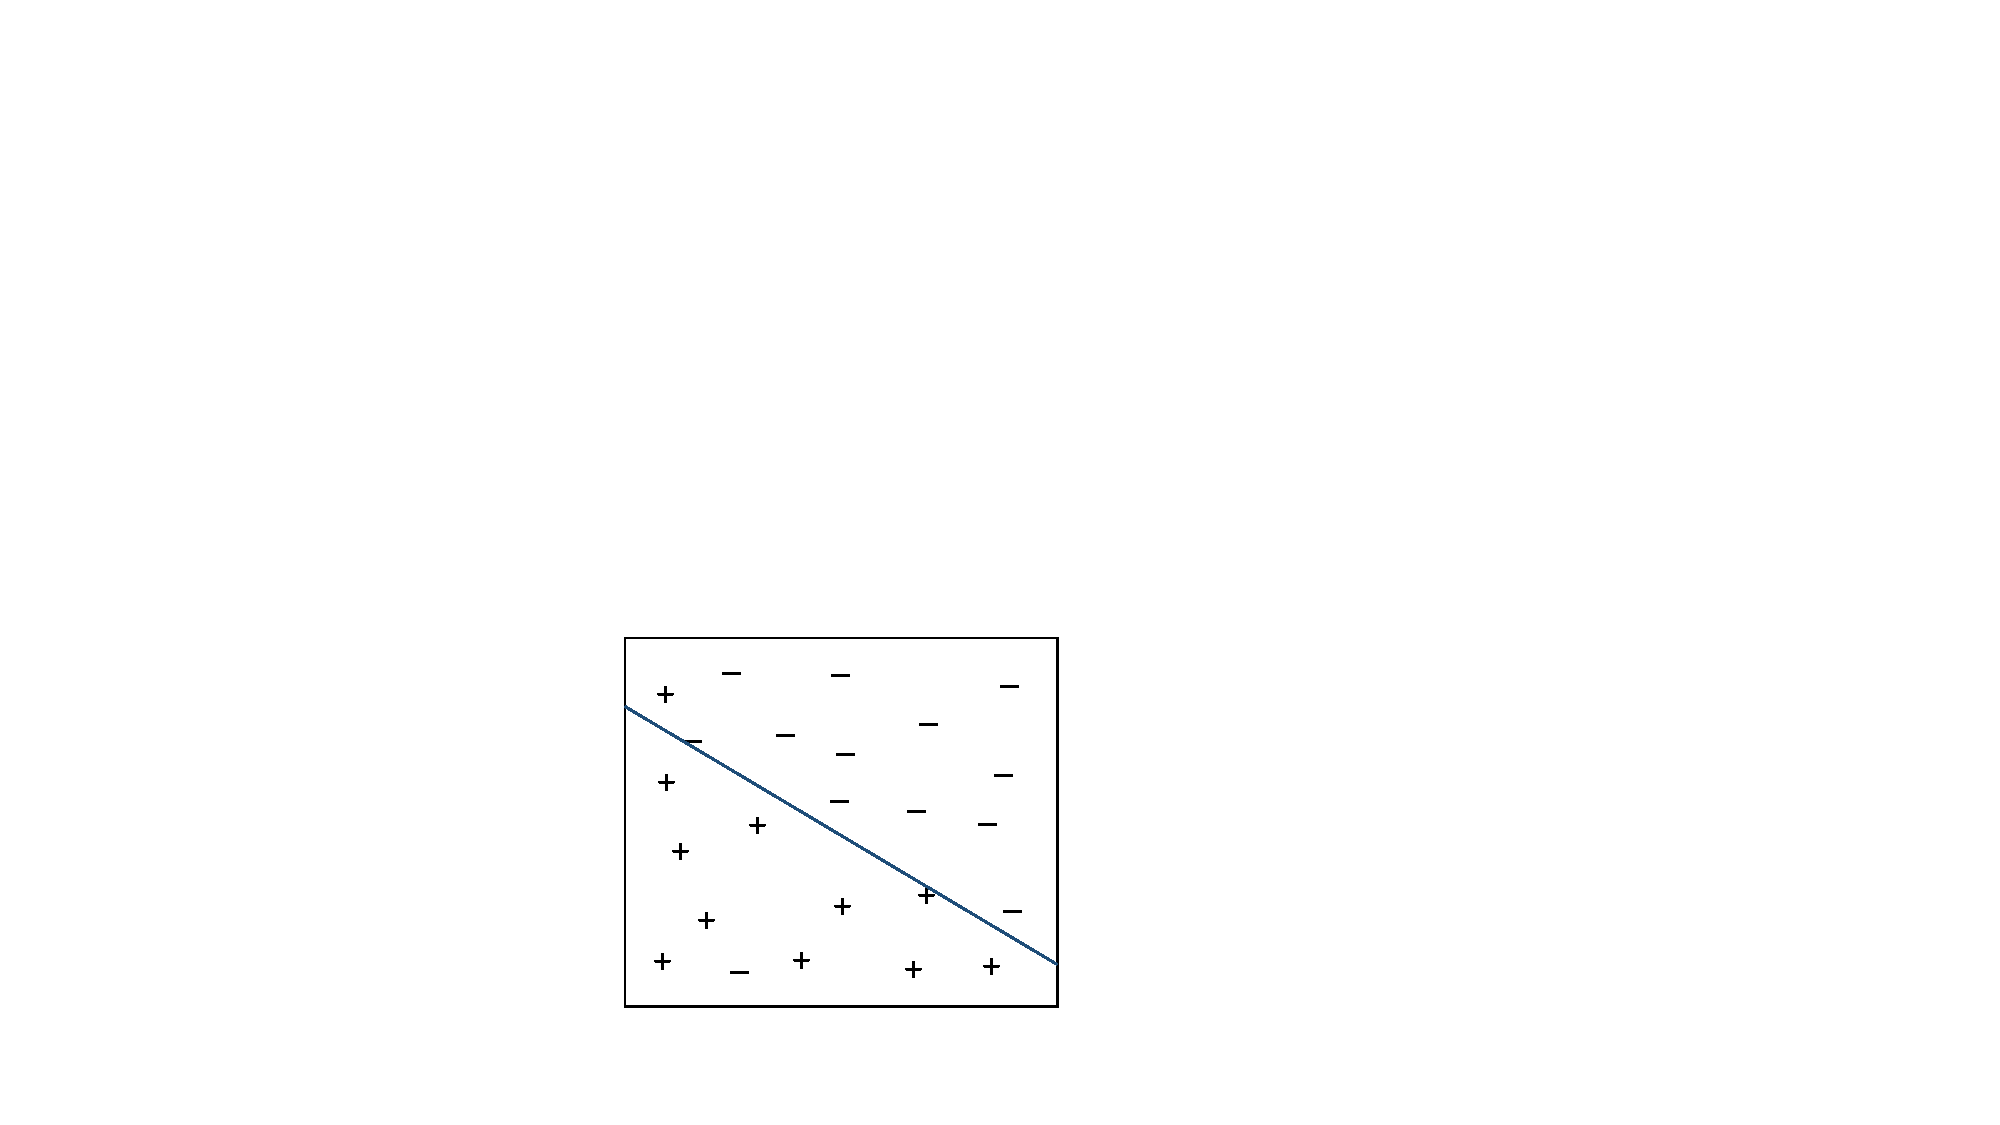
\includegraphics{figs/condrift-a.pdf}} &
            \resizebox{60mm}{!}{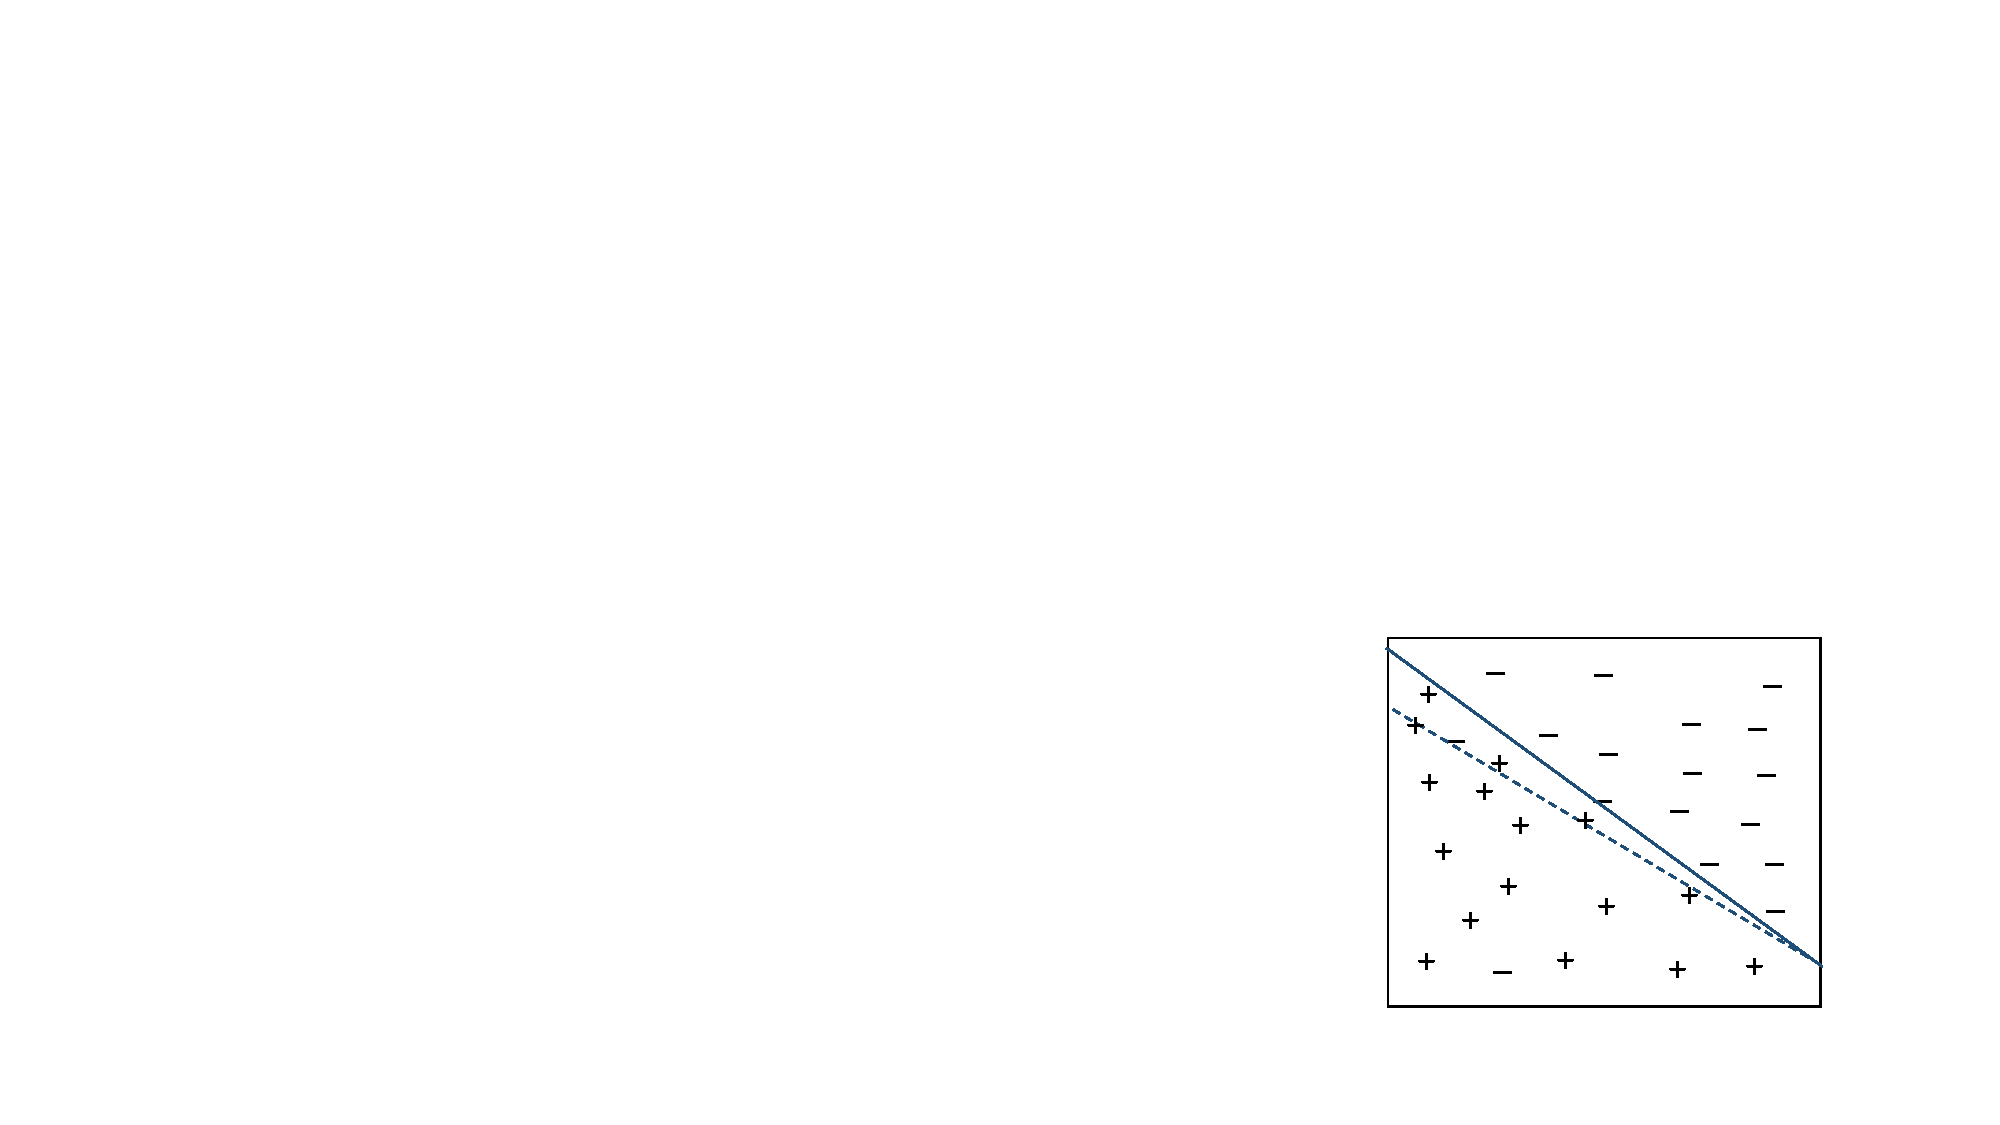
\includegraphics{figs/condrift-b.pdf}} \\
            \scriptsize{(a)\hspace{0mm}} & \scriptsize{(b)}    
        \end{tabular}
    \caption{Concept drift in data streams}
    \label{fig:bg:condrift}
    \end{center}
\end{figure}
\paragraph{Concept drift:}
Concept drift is a statistical property of data streams where the target variable drifts away from the model that is trying to predict it. In other words the underlying data distribution is changing over time. As a result, accuracy of the classifier model decreases over time. For example, buying pattern of the customers in a store changes over time, mostly due to the seasonality. Electrical and mechanical devices wear off over time, producing shifted result which would cause drift in the observing data. Learning models should adapt to these changes quickly and accurately. Let us consider the example in Figure~\ref{fig:bg:condrift}. As a new chunk arrives (Figure~\ref{fig:bg:condrift}a), a new classifier is learned. The decision boundary is denoted by the straight line. The positive examples are represented by pluses while the negative examples are represented by minuses. With time the concept of some of the examples may change. As shown in Figure~\ref{fig:bg:condrift}b, due to concept drift newer positive examples may drift towards decision boundary and into negative concept's region. So, the previous decision boundary has become outdated and the model has to be updated. Formally, concept drift is the change in the joint probability \(P(X, y) = P(y|X) \times P(X)\). Thus, observing the change in $y$ for given $X$, i.e. $P(y|X)$ is the key for detecting concept drift.

One challenge posed here is to differentiate between the noise in data and the actual shift in the concept. Often in streaming environment data contain the both. Rate of drift is also a factor in detection. Sudden drift, known as {\it concept shift}, is easier to detect than concept drift, which is considered to be gradual.

\begin{figure}[htbp]
    \begin{center}
        \begin{tabular}{cc}
            \resizebox{60mm}{!}{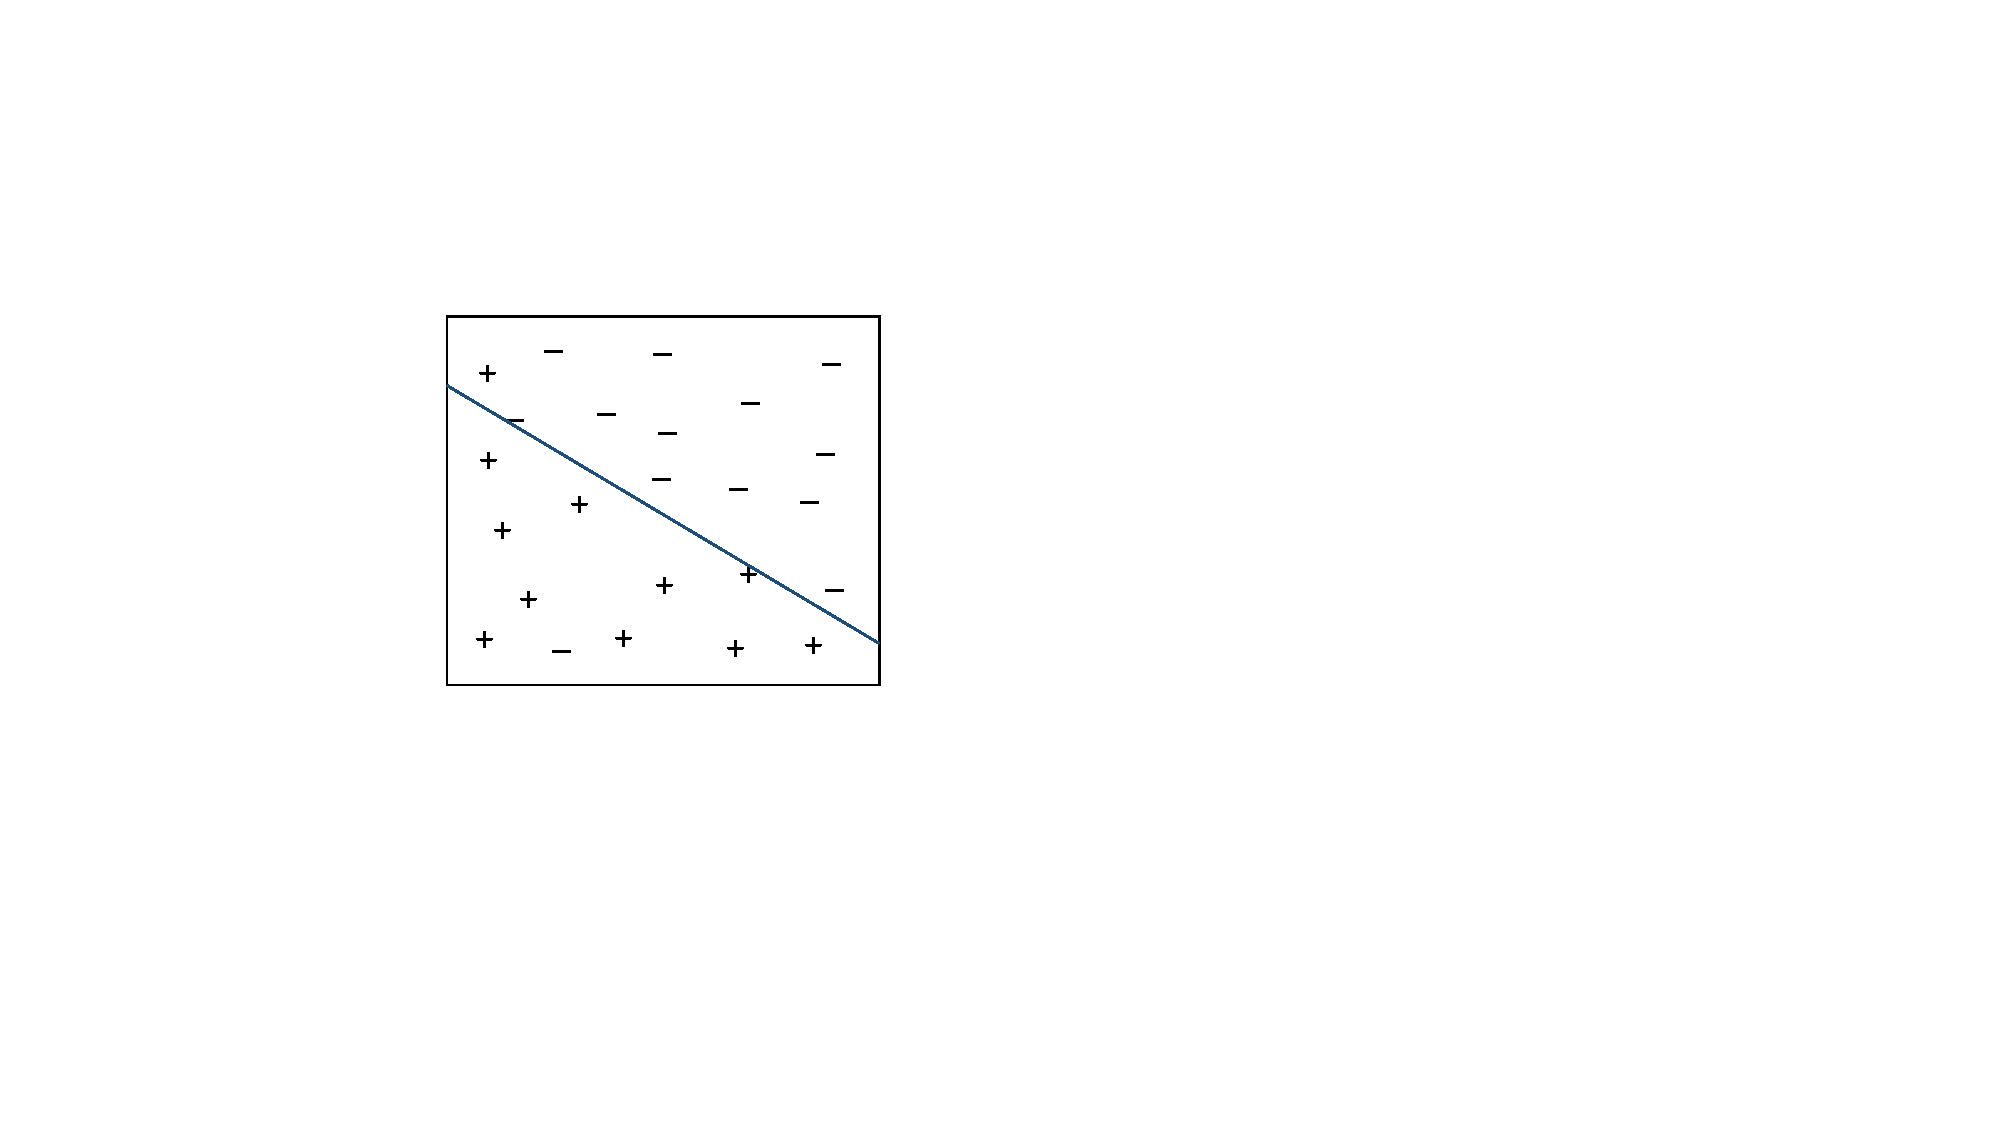
\includegraphics{figs/conevol-a.pdf}} &
            \resizebox{60mm}{!}{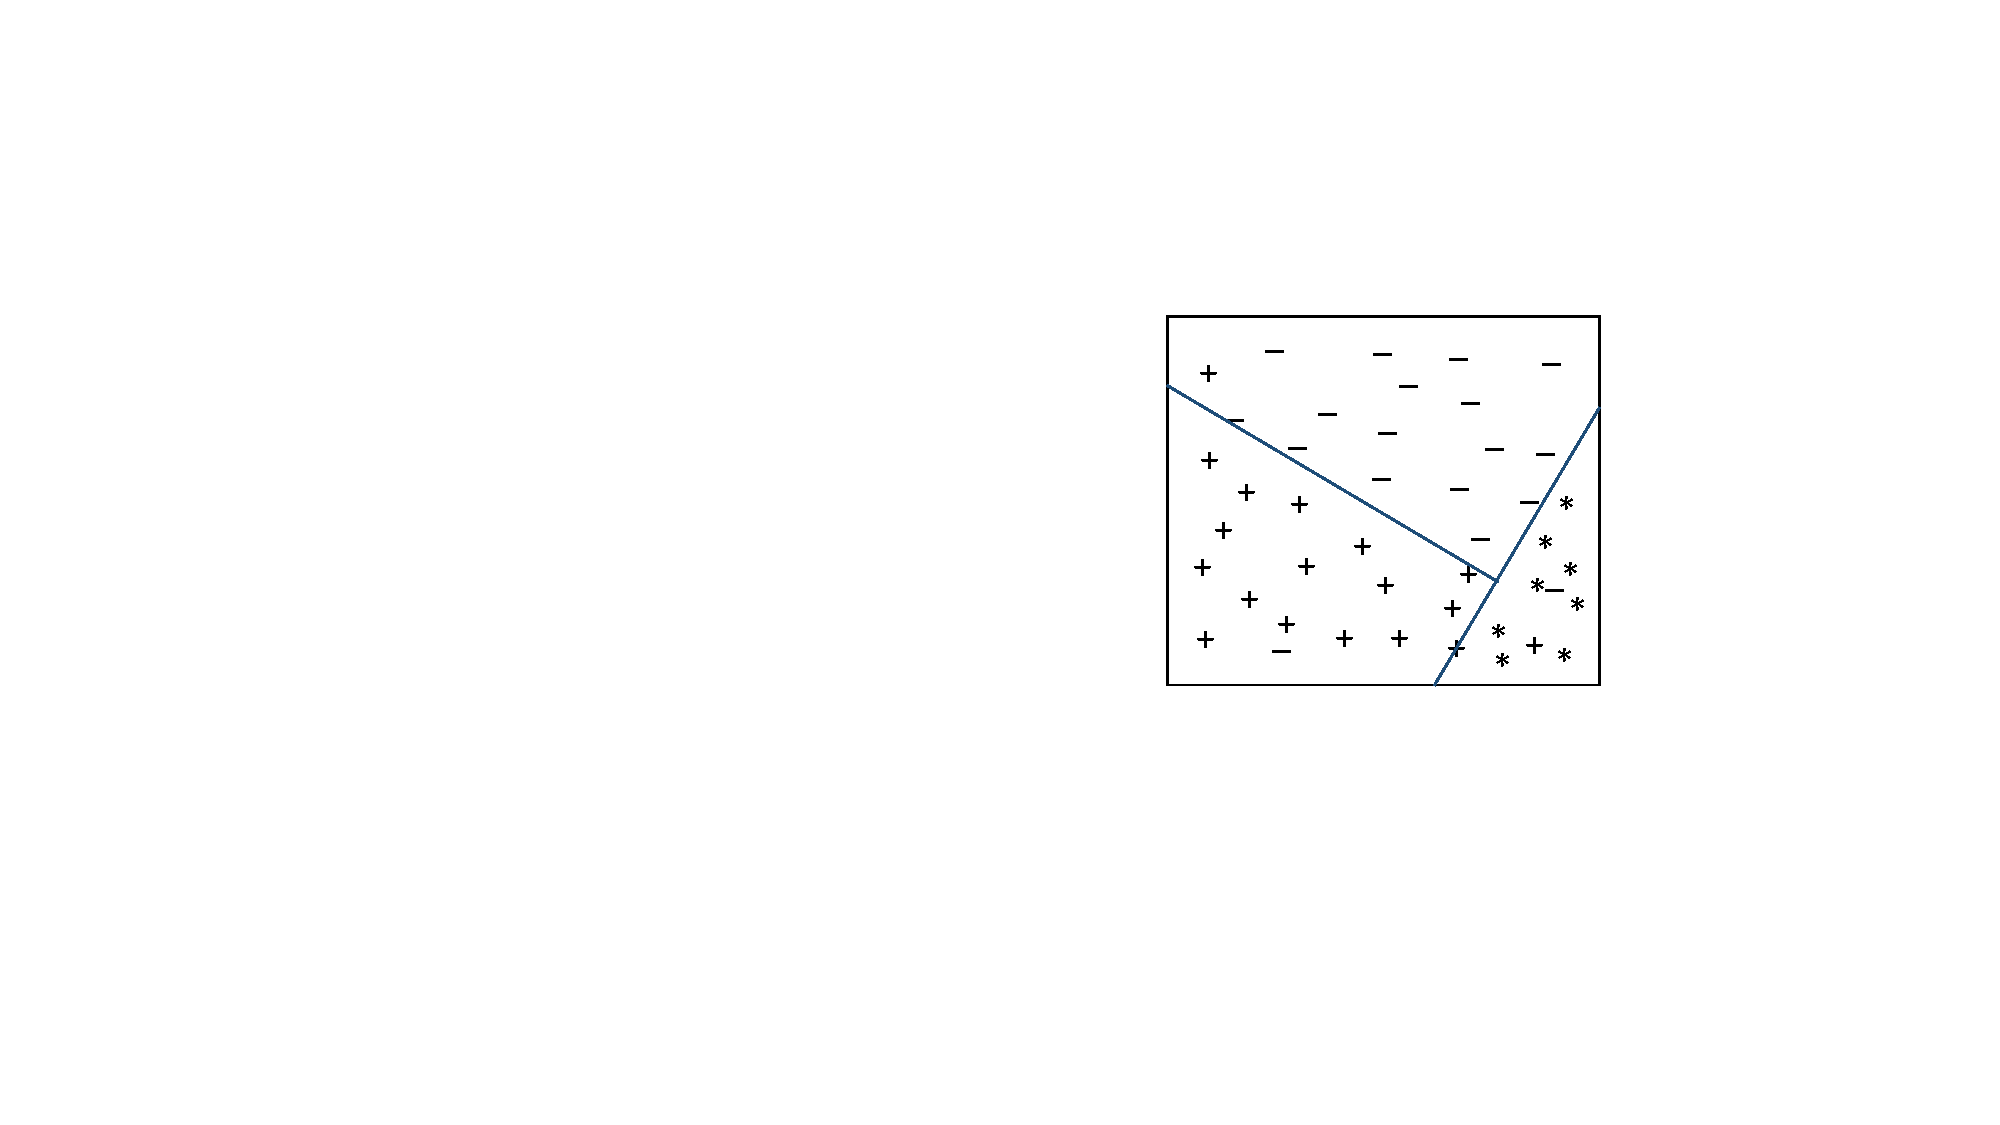
\includegraphics{figs/conevol-b.pdf}} \\
            \scriptsize{(a)\hspace{0mm}} & \scriptsize{(b)}    
        \end{tabular}
        \caption{Concept evolution in data streams.}
        \label{fig:bg:dataevol}
    \end{center}
\end{figure}
\paragraph{Concept evolution:}
Concept evolution is referred to the emergence of a new class or a set of classes in stream data as the time passes. Twitter stream is an ideal example where concept evolution is easily identifiable. Twitter reacts, seemingly, very fast upon important news around the globe. Looking into the different hash tag usages in such social media currently trending topics can be identified. To present a clearer picture let's consider following example in Figure~\ref{fig:bg:dataevol}. For a certain point of time two classes and their corresponding decision boundaries are shown in the Figure~ \ref{fig:bg:dataevol}a. With the more incoming data a novel class emerges, and for that decision boundaries need updating. Emergence of new class can affect any number of decision boundaries/ rules, from one to all. 
Concept evolution is also prone to noise. Furthermore, clear distinction between drift and evolution might not always be possible, partially due the lack of unlabeled data.

\paragraph{Class recurrence:}
Class recurrence is a special case of concept drift and evolution. In this case, the model forgets a class due the drift or absence of data for some period, however, later the class reappears (evolution) in the stream. Seasonality could be one cause of this situation. An intrusion in network traffic may reappear after a long time. Forgetting the earlier intrusions are not desired in such case. A fast recognition of the previously seen classes are desired in stream mining.

Following sections discuss the potential solutions to these challenges. First, how to address the limited resources and then the change detection schemes.

\subsection{Maintaining Sufficient Statistics}
In statistical evaluation, a statistic is sufficient for a family of probability distributions if the sample from which it is calculated gives no additional information than does the statistic, as to which of those probability distributions is that of the population from which the sample was taken~\cite{fisher22:suffstat}. Mathematically, given a set  $\mathbf{X}$ of independent identically distributed data conditioned on an unknown parameter $\theta$, a sufficient statistic is a function $T(\mathbf{X})$ whose value contains all the information needed to compute any estimate of the parameters (e.g. maximum likelihood estimate). Using the factorization theorem (Theorem~\ref{thm:factor}), for a sufficient statistic $T(\mathbf{X})$, the joint distribution can be written as $ p(\mathbf{X}) = h(\mathbf{X}) g(\theta, T(\mathbf{X}))$. From this factorization, it can easily be seen that the maximum likelihood estimate of $\theta$ will interact with $\mathbf{X}$ only through $T(\mathbf{X})$. Typically, the sufficient statistic is a set of function or random variables of the data.

\begin{theorem}[Factorization Theorem]
    \label{thm:factor}
    Let $X_1, X_2, \dots , X_n$ be a random sample with joint density $f(x_1, x_2, \dots , x_n| \theta)$. A statistic $T = r(X_1, X_2, \dots , X_n)$ is sufficient if and only if the joint density can be factored as follows:
    \[
    f(x_1, x_2, \dots , x_n| \theta) = u(x_1, x_2, \dots , x_n) v(r(x_1, x_2, \dots , x_n), \theta)
    \]
    where $u$ and $v$ are non-negative functions. The function $u$ can depend on the full random sample $x_1, x_2, \dots , x_n$, but not on the unknown parameter $\theta$. The function $v$ can depend on $\theta$, but can depend on the random sample only through the value of $r(x_1, x_2, \dots , x_n)$.
\end{theorem}

\subsubsection{Bounds of Random Variable}
A random variable is a variable that can take a set or range of values, each with an associated probability, and is subjected to change due to the alteration or randomness of the data. Random variables are of two types: (i) discrete, and (ii) continuous. Discrete random variable takes a set of possible values (e.g. outcome of coin flipping), but a continuous random variable can take any value within a range (e.g. age of people in a randomly sampled group).

A function that is used to estimating a random variable is called an estimator. Estimator function is dependent on the observable sample data, and used for estimating unknown population within an interval with certain degree of confidence. For an interval of the true values of the parameter associates with a confidence of $1 - \delta$, interval can be defined as follows:
\begin{itemize}    
    \item Absolute approximation: $\bar{X} - \epsilon \le \mu \le \bar{X} + \epsilon$, where $\epsilon$ is the absolute error.
    \item Relative approximation: $(1 - \delta)\bar{X} \le \mu \le (1 + \delta)\bar{X}$, where  is the relative error.
\end{itemize}
where $\mu$ and $\bar{X}$ represent actual and estimated mean. There are a number of theorems that provide bounds on the estimation, Chebyshev, Chernoff, Hoeffding bounds~\cite{hoeffding63:bound}, etc. are few of them.

\begin{theorem}[Chebyshev Bound]
\label{thm:chebyshev}
    Let $X$ be a random variable with standard deviation $\sigma$, the probability that the outcome of $X$ is no less than $k\sigma$ away from its mean is no more that $1/k^2$:
    \[
        P(|X-\mu| \le k\sigma) \le \frac{1}{k^2}
    \]
    In other words, it states that no more that $1/4$ of the values are more than $2$ standard deviation away, no more than $1/9$ are more than $3$ standard deviation away, and so on.
\end{theorem}

\begin{theorem}[Chernoff Bound]
\label{thm:chernoff}
    Let $X_1,X_2,\dots, X_n$ be independent random variables from Bernoulli experiments. Assuming that $P(X_i = 1) = p_i$. Let $X_s = P_n \sum_{i=1}{n} X_i$ be a random variable with expected value $\mu_s = P \sum_{i=1} np_i$. Then for any $\delta > 0$:
    \[
        P[X_s > (1+\delta) \mu_s] \le (\frac{e^\delta}{(1 + \delta)^{1 +\delta}} )  ^{\mu_s}
    \]
    and the absolute error is:
    \[
        \epsilon \le \sqrt{\frac{3 \bar{\mu}}{n} \ln (2/\delta)}
    \]
\end{theorem}

\begin{theorem}[Hoeffding Bound]
\label{thm:hoeffding}
    Let $X_1,X_2,\dots, X_n$ be independent random variables. Assuming that each $x_i$ is bounded, that is $P(X_i \in R = [a_i, b_i]) = 1$. Let $S = 1/n \sum_{i=1}{n} X_i$ whose expected value is $E[S]$. Then, for any $\epsilon > 0$:
    \[
        P[S - E[S] > \epsilon] \le e^{ \frac{2 n^2 \epsilon^2}{R^2} }
    \]
    and the absolute error is:
    \[
        \epsilon \le \sqrt{\frac{R^2 \ln(2/\delta)}{2n}}
    \]
\end{theorem}

Chernoff and Hoeffding bounds are independent of the underlying distribution of examples. They are more restrictive or conservative, and require more observations as compared to the distribution dependent bounds. Chernoff bound is multiplicative and Hoeffding is additive. They are expressed as relative and absolute approximation, respectively.

These methods only take a finite number of values or a range. One of the well-known methods supports infinity is Poisson process. A random variable $x$ is Poisson random variable with parameter $\lambda$ if $x$ takes values $0,1,2, \dots, \infty$ with:
    \begin{equation}
    \label{eqn:poisson}
        p_k = P(x=k) = e^{-\lambda} \frac{\lambda^k}{k!}
    \end{equation}
where, $\lambda$ is both mean and variance, i.e. $E(X) = Var(X) = \lambda$.
    
\subsubsection{Recursive Mean, Variance, and Correlation}
Fundamental equations of mean, variance, etc. are not usable for streams as past data points are lost as the time passes. However, their recursive versions can easily be derived. Equation~\ref{eqn:mean}, \ref{eqn:var}, and \ref{eqn:corr} can be used to recursively compute mean, variance, and correlation respectively.

\begin{equation}
\label{eqn:mean}
    \bar{x}_i = \frac{(i-1) \times \bar{x}_{i-1} + x_i}{i}
\end{equation}

\begin{equation}
\label{eqn:var}
    \sigma_i = \sqrt{ \frac{\sum x_i^2 - \frac{ (\sum x_i )^2}{i} }{i-1} }
\end{equation}

\begin{equation}
\label{eqn:corr}
    corr(a, b) = \frac{ \sum(x_i \times y_i) - \frac{\sum x_i \times \sum y_i}{n} }{\sqrt{\sum x_i^2 - \frac{\sum x_i^2}{n}} \sqrt{\sum y_i^2 - \frac{\sum y_i^2}{n}}}
\end{equation}

As it can be seen from the equations, maintaining (i) number of observations, $n$; (ii) $\sum x_i$, sum of $i$ data points; (iii) $\sum x_i^2$, sum of squares of $i$ data points; and (iv) $\sum (x_i \times y_i)$, sum of cross product of $X$ and $Y$ are enough to recursively compute these statistics.


\subsubsection{Windowing}
Windowing is the process of selecting a subset of the observed instances that would be remembered to be used in the computation of statistics. Where the data set is finite and of limited size, all the instances can be remembered. For streams, this is not possible. Furthermore, computing statistics over all the instances of the past, in streaming environment, would wrongly introduce information of classes that are not currently present. Thus, information of recent past is more important than the entire set. Windowing is categorized in two basic types: (i) sequence based windowing, and (ii) timestamp based windowing.

In sequence based windowing, sequence is based on the number of observations seen; in timestamp based approach, it is elapsed time. Landmark windowing and sliding windowing are the two most used sequence based windowing system.

\paragraph{Landmark Windowing:} All observations after certain start point are remembered. Batched approaches can be thought of as examples of landmark windowing where every instance is remembered from the very first one. As new observations are seen, size of window increases. Landmark needs updating to ensure that the statistics are recent.

\paragraph{Sliding Windowing:} A fixed length window is moved through the observation set. As a new observation is seen, the oldest observation is forgotten, i.e., when $j$-th instance is pushed into the window, $(j-w)$-th instance is forgotten, where $w$ is the size of the window. A limitation of sliding windowing is that it requires all elements within the window to be remembered, as it  needs to forget the oldest observation.

Often it is more useful to learn about most recent updates with fine granularity and older ones in a summarized fashion. With this motivation concept of tilted-time windowing was introduced~\cite{chen02:tiltedtime}.

\begin{figure}[htbp]
    \begin{center}
        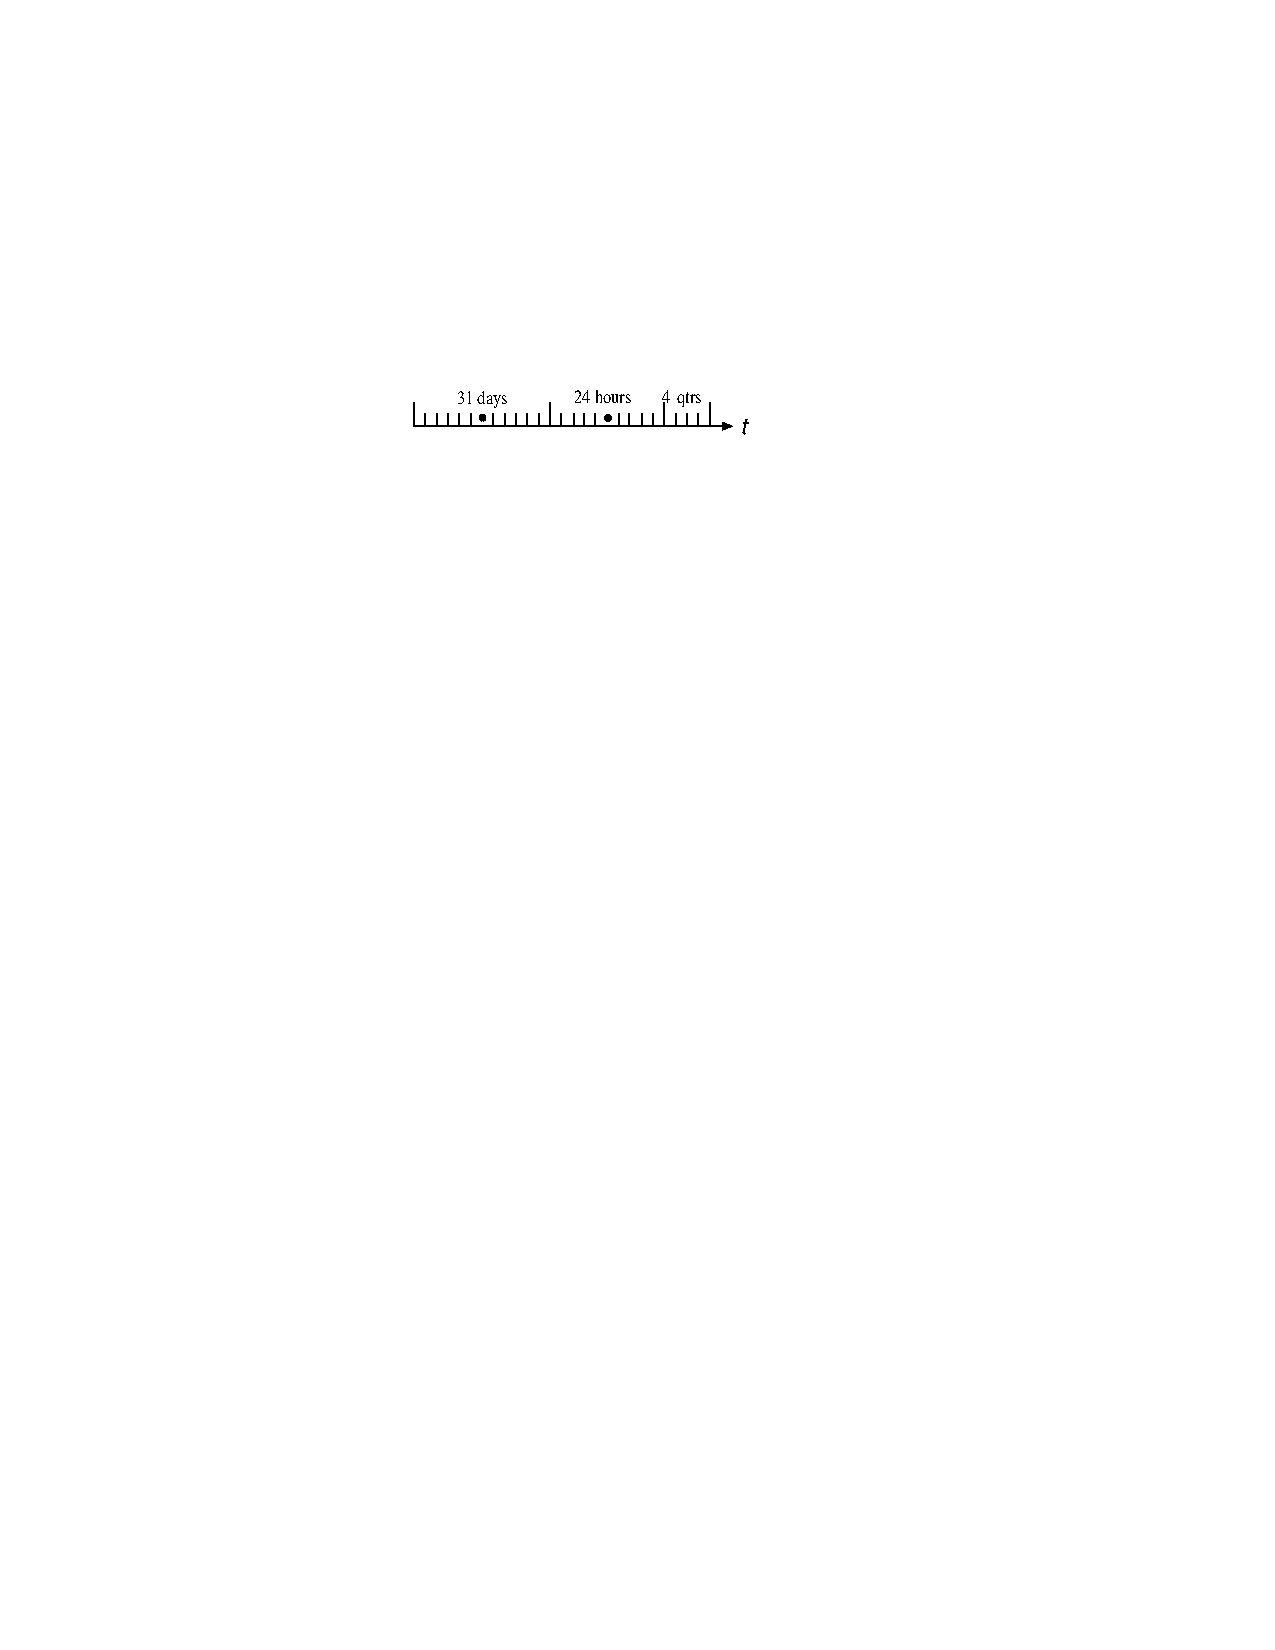
\includegraphics[width=3.0in]{figs/naturaltime.pdf}
        \caption{Natural Tilted Time Window}
        \label{fig:bg:ntime}
    \end{center}
\end{figure}
\paragraph{Natural Tilted Time Windowing:} In natural tilted time windowing, units of time is distributed non-uniformly. Most recent time gets more units. For example, Figure~\ref{fig:bg:ntime} shows a natural tilted time windowing scheme, where for most recent hour, quarterly updates are stored in 4 units. Similarly, 24 units of time storing a day's, and 31 units storing a months' summary. That is, with 59 units of time information, this model stores about 32 days' information.

\begin{figure}[htbp]
    \begin{center}
        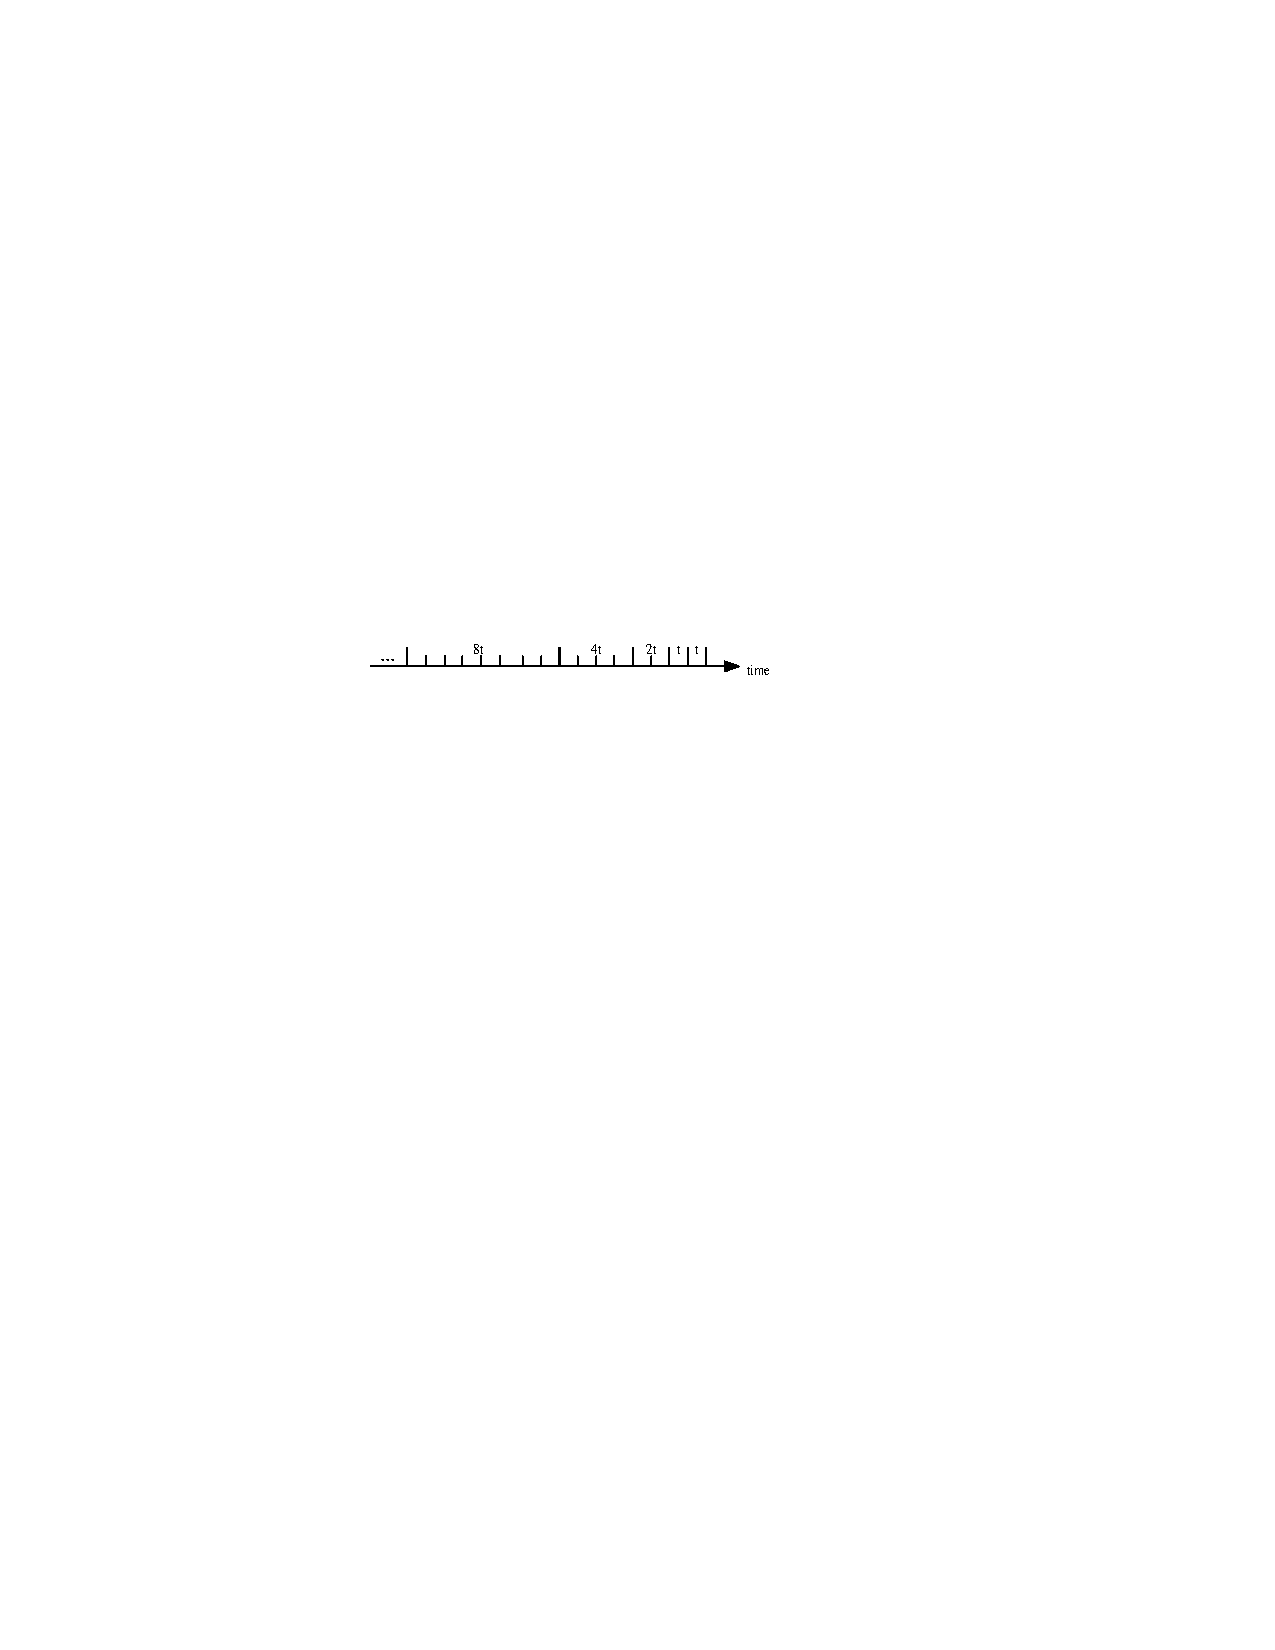
\includegraphics[width=4.0in]{figs/logtime.pdf}
        \caption{Logarithmic Tilted Time Window}
        \label{fig:bg:ltime}
    \end{center}
\end{figure}
\paragraph{Logarithmic Tilted Time Windowing:} Concept for logarithmic tilted time windowing is same as natural tilted time windowing. The only deference here is that time scale grows in logarithmic order. Figure~\ref{fig:bg:ltime} shows an example. 


\subsection{Change Detection}
\label{sec:bg:changedetection}
An assumption of most machine learning methods is that data are generated from a stationary distribution. As discussed in the previous section, this assumption does not hold for streaming scenario. Thus stream mining requires algorithms to facilitate drift detection methods. Differentiating between {\it noise} and {\it change} makes the problem challenging. The difference between a new distribution and noise is {\it persistence}, where new examples consistently follows new distribution rather than old. This section discusses several methods to detect and adapt learning algorithms in presence of concept drift.

Detection methods can generally be classified into two categories. First approach is to monitoring the evolution of various performance indicators as done in~\cite{klinkenberg98:changedetection, zeira04:changedetection}. Another approach is to maintaining two (or more) distributions varying the window length. Typically, one window would summarize past history while the other would summarize most recent information~\cite{kifer04:condrift}.

Most methods follow the first approach. \cite{klinkenberg98:changedetection} monitors three performance indicators (accuracy, recall, and precision) over time, and uses their posterior comparison to a confident interval of standard sample errors for a moving average value for each indicator.

A classical algorithm for change detection is \textit{Cumulative Sum (CUSUM)}~\cite{page54:cusum}. CUSUM can detect that the mean of the input data is significantly different than zero. The test is as follows:
\[
    g_0 = 0 
\]\[
    g_t = max (0, g_{t-1} + (r_t - v))
\]
If $g_t > \lambda$, CUSUM triggers an alarm and set $g_t = 0$. This detects the changes in the positive direction. To detect the negative change $min$ is used instead of $max$. CUSUM does not require any memory. Its accuracy depends on the choice of $v$ and $\lambda$. Low $v$ results in faster detection with more false positives.

For latter category, \cite{kifer04:condrift} uses Cherfnoff bound (Theorem~\ref{thm:chernoff}) and examines examples drawn from two probability distributions and decides whether these distributions are different.

\paragraph{ADWIN Algorithm:} ADWIN (ADaptive sliding WINdow) is another change detection algorithm of latter type. ADWIN keeps a variable length window of recent items. It ensures the property {\it there has been no change in the average value inside the window} for maximally statistically consistent length. The core idea of ADWIN is that whenever two {\it large enough} sub-windows of $W$ exhibit {\it distinct enough} averages, it is assumed that their corresponding expected values are different, and the older portion of the window is dropped. Essentially, this means that when the difference of means of the two windows is greater than a certain threshold $\epsilon_{cut}$, the older portion should be dropped. Equation to compute $\epsilon_{cut}$ is as follows:
\[
    m = \frac{2}{1/|W_0| + 1/|W_1|}
\]\[
    \epsilon_{cut} = \sqrt{\frac{1}{2m} \ln \frac{4 |W|}{\delta}}
\]
where $\delta \in (0, 1)$ is confidence value, an input.

\begin{algorithm}[htbp]
    \DontPrintSemicolon
\label{alg:adwin}
\caption{ADWIN Algorithm}

    \KwData{Data Stream}
    \KwResult{Window with most recent concept}
    \Begin{
        Initialize window $W$ \\
        \ForEach{$t > 0$} {
            $W \leftarrow W \cup \{x_t\}$ \tcp*[f]{add $x_t$ to the head of $W$ }\\
            \Repeat{$|\mu_{W_0} - \mu_{W_1}| < \epsilon_{cut}$ holds for every split of $W$} {
                Drop element from the tail of W\\
            }
            $W = W_0 . W_1$\\
        }
        Output $\mu_W$\\
    }
\end{algorithm}

ADWIN does not maintain the windows explicitly, but compresses it using a variant of the exponential histogram technique. This means that it keeps a window of length $w$ using only $O(\lg w)$ memory and $O(\lg w)$ processing time per item.

\subsubsection{Adaptation to Change}
To improve accuracy of a decision model under concept drifting environment, decision model needs adaptation to the changes. There are two types of approaches based on when to adapt: 
\begin{itemize}    
    \item Blind or periodic methods: Models are updated on regular interval whether any change has actually occurred or not. 
    \item Informed methods: Models are only updated when there are sufficient reasons to believe that changes in the concept have occurred.
\end{itemize}
It could be a good idea to use periodic methods where duration of the seasonality is known beforehand. Otherwise, chosen duration could be too large or too small to response to the changes. In such cases, an informed decision is more desired. However, informed methods requires more resources (than blind methods) to be able to make such decision.

\subsection{Na\"ive Bayes Adaptation}
Na\"ive Bayes algorithm is essentially a stream classification algorithm. One of the advantages of this classifier in the context of data stream is its low complexity for deployment. It only depends on the number of explanatory variables. Its memory consumption is also low since it requires only one conditional probability density estimation per variable.

\begin{algorithm}[htbp]
    \caption{VFDT: The Hoeffding Tree Algorithm}
    \label{alg:vfdt}
    \DontPrintSemicolon
    \SetKwInOut{Input}{Input} \SetKwInOut{Output}{Output} 
    
    \Input{$S$: Stream of examples \\
        $X$: Set of nominal attributes \\
        $Y$: Set of class labels $Y = \{y_1, y_2, \dots, y_k\}$ \\
        $G(.)$: Split evaluation function \\
        $N_{min}$: Minimum number of examples \\
        $\delta$: is one minus the desired probability \\
        $\tau$: Constant to resolve ties
    } 
    \Output{$HT$: is a decision tree}
    
    \Begin{
        Let $HT \leftarrow$ Empty Leaf (Root)
        \ForEach{$example(x, y_k) \in S$} {
            Traverse the tree $HT$ from root till a leaf $l$ \\
            
            \eIf (\tcp*[f]{Missing class label}) {$y_k == ?$ } {
                Classify with majority class in the leaf $l$
            } {
                Update sufficient statistics \\
                \If{$ Number\;of\;examples\;in\;l > N_{min}$ }{
                    Compute $G_l(X_i)$ for all attributes \\
                    Let $X_a$ be the attribute with highest $G_l$ \\
                    Let $X_b$ be the attribute with second highest $G_l$ \\
                    Compute $\epsilon = \sqrt{\frac{R^2 \ln(2/\delta)}{2n}}$  \tcp*[f]{Hoeffding bound} \\
                    
                    \If{$G(X_a) - G(X_b) > \epsilon\; || \;\epsilon < \tau$} {
                        Replace $l$ with a splitting test based on attribute $X_a$ \\
                        Add a new empty leaf for each branch of the split \\
                    }
                }
            }
        }
        Return $HT$
    }

\end{algorithm}

\subsection{Very Fast Decision Tree}
\label{sec:bg:vfdt}
Very Fast Decision Tree (VFDT), also known as Hoeffding Tree (HT), is a decision tree based adaptation for streams generating from a stationary distribution. It is an anytime-ready algorithm and uses Hoeffding bound to ensure the performance in terms of accuracy is asymptotically nearly identical to that of conventional tree based algorithms. VFDT runs on constant time and memory per examples and can serve thousands of examples on a typical consumer system.

VFDT constructs the tree by recursively replacing leaves with decision nodes. Each leave stores sufficient statistics that are required to evaluate the merit of split-test and to decide the target class. For incoming instances, the tree is traversed from the root to a leaf (based on the incoming instance's values) and the statistics are updated accordingly. If a unanimous decision cannot be reached based on observed instances at any particular leaf node, the node is tested to check the sufficiency for a split. If there is enough statistical support in favor of a split, the node is splitted on the best attribute and stats are passed to the descendants (new leaves). Number of descendants of this new decision node is equal to the number of possible values of the chosen attribute. Thus, the tree is not necessarily a binary tree.

Deciding on whether to split a node or not is a unique contribution of VFDT. VFDT solves this difficult problem of deciding exactly how many examples are required to be observed by a leaf node before splitting by using Hoeffding bound (Theorem~\ref{thm:hoeffding}). Let $G(.)$ be the heuristic measure of the attributes. This measure could be information gain as of C4.5 or Gini index of CART. For information gain, range $R$ in Hoeffding bound is $\lg (\#classes)$. Goal is to find a $n$ such that the attribute chosen for split after observing $n$ instances would, with high probability, be the same as it would be chosen after observing infinite instances. Assume that $X_a$ is the attribute with the best $G(.)$, and $X_b$ is the second best attribute after observing $n$ instances. Then $\Delta G = G(X_a) - G(X_b)$ is the difference between their observed heuristics. From Hoeffding bound, we know if $\Delta G > \epsilon$, then with probability $1 - \delta$, $X_a$ would be the attribute with highest value in the evaluation function in the universe. Otherwise, if $\Delta G < \epsilon$, then the sample size is not enough to make a stable split decision. As the assumption is that underlying generating distribution is stationary, thus as the sample size increases, $\epsilon$ decreases and heuristic value for most informative attribute goes up.

To fasten up the process, VFDT uses an extra parameter $N_{min}$ to reduce the number of $G(.)$ computation. Computing $G(.)$ when there are too few instances is run-time inefficient. Thus a user parameter $N_{min}$ is used to indicate minimum number of instances needed to be observed before the evaluation starts. This is known as grace period.

When multiple attributes continuously perform similar in heuristic evaluation after observing a large number of examples, $\Delta G$ might never be greater than $\epsilon$. To break such tied cases, another user parameter $\tau$ is used, and when $\epsilon$ falls below $\tau$ (i.e. $\Delta G < \epsilon <\tau$), algorithm splits on the best attribute. Algorithm~\ref{alg:vfdt} summarizes the pseudo-code of VFDT.

There are some properties of VFDT that are different than C4.5. In contrast to the C4.5 algorithm number of examples that support a decision increases in VFDT. Typically VFDT also results a lower variance model than that of C4.5. However, there is no mechanism avoid over-fitting in VFDT as there is no room for pruning.

\begin{algorithm}[htbp]
    \DontPrintSemicolon
    \SetKwInOut{Input}{Input} \SetKwInOut{Output}{Output} 
    \caption{CVFDT: Concept-adapting VFDT}
    \label{alg:cvfdt}
    
    \Input{$S$: Stream of examples \\
        $X$: Set of nominal attributes \\
        $Y$: Set of class labels $Y = \{y_1, y_2, \dots, y_k\}$ \\
        $G(.)$: Split evaluation function \\
        %$N_{min}$: Minimum number of examples \\
        $\delta$: is one minus the desired probability \\
        $\tau$: Constant to resolve ties \\
        $w$: Size of the window \\
        $n_{min}$: Number of examples between checks for growth \\
        $f$: Number of examples between checks for drift
    } 
    \Output{$HT$: is a decision tree}
    
    \Begin{
        Let $HT \leftarrow$ Empty Leaf (Root) $l_0$ \\
        Let $Alt(l_0) \leftarrow \emptyset$ \tcp*[f]{Alternate trees for $l_0$} \\
        %Let $G(X_\emptyset)$ be the $G(.)$ obtained by predicting most frequent class \\
        %Let $X_1 = X \cup \{X_\emptyset\}$ \\
        
        \ForEach{class $y_k$} {
            \ForEach{$x_{ij} \in X_i \in X$} {
                Set $n_{ijk} = 0$
            }
        }
        \ForEach{$example(x, y) \in S$} {
            Traverse the tree $HT$ including $Alt(\{n: (x,y)\;passes\;through\;n\;in\;HT\})$ trees root till a set of leaves $L$ \\
            
            Set $id = \max(\{L.id\})$ \\
            Add $((x, y), id)$ to the beginning of $W$ \\
            \If{$|W| > w$} {
                Let $((x_w, y_w), id_w)$ be the last element in $W$ \\
                FORGET($HT, n, (x_w, y_w), id_w)$) \label{algln:cvfdt:forget} \\
                $W = W - ((x_w, y_w), id_w)$
            }
            GROW($HT, n, G, (x,y)$ \\
            \If{examples seen since last checking $> f$}{
                VALIDATE\_SPLIT($n$) \label{algln:cvfdt:validatesplit} 
            }
        }
        Return $HT$
    }
\end{algorithm}
\subsection{Concept-adapting Very Fast Decision Tree}
Concept-adapting Very Fast Decision Tree (CVFDT) is the extension of CFDT that adds the ability to adapt the model by detecting the changes in the underlying distribution that generates the examples. CVFDT does not require the model to be recomputed, instead it updates the sufficient statistics stored in each node that the new instances affects by maintaining a sliding window. It increases the counter of new instances and decreases count of the oldest examples which now needs an instance to be forgotten. If the underlying distribution is stationary, this would not have any effect. But in case of a concept drifting distribution, some decision nodes that previously had passed the Hoeffding bound test will no longer pass, rather an alternate attribute would now have higher or similar gain. CVFDT keeps stats to detect such situation and starts maintaining an alternate subtree with the new best attribute as its root. When this alternate subtree becomes more accurate on new data, then the old subtree is replaced by the new one. Pseudo-code of CVFDT has been shown in Algorithm~\ref{alg:cvfdt}. The sub-routine $GROW$ is essentially the Hoeffding Tree algorithm where instead of only keeping stats in the leave, every node keeps track of the instances it has seen. Two other sub-routines $FORGET$ and $VALIDATE\_SPLIT$ have been shown separately.

\begin{algorithm}[htbp]
    \ContinuedFloat
    \DontPrintSemicolon
    \LinesNumberedHidden
    \setcounter{algoline}{0}
    \newcommand\Numberline{\refstepcounter{algoline}\nlset{\thealgoline}}
    \SetNlSty{textbf}{\ref*{algln:cvfdt:forget}.}{}
    
    \SetKwInOut{Input}{Input} \SetKwInOut{Output}{Output} 
    \SetKwInOut{TitleOfAlgo}{Algorithm}
    \TitleOfAlgo {FORGET($HT, n, (x_w, y_w), id_w$)}
    \label{alg:cvfdt:forget}
    
    \Begin{
        \Numberline Sort $(x_w, y_w)$ through $HT$ while it traverses leaves with $id \le id_w$ \\
        \Numberline Let $P$ is the set of sorted nodes \\
        
        \Numberline \ForEach{node $l \in P$} {
        \Numberline     \ForEach{$x_{ij} \in x : X_i \in X_l$} {
        \Numberline         Decrement $n_{ijk}(l)$
            }
        \Numberline     \ForEach{tree $t_{alt} \in Alt(l)$} {
        \Numberline         FORGET($t_{alt}, n, (x_w, y_w), id_w$)
            }
        }
    }
\end{algorithm}

$FORGET$ function is used to remove the effect of instances of older concepts. However, this is not straight-forward as HTs go through changes after the instance to be forgotten was initially added. Thus, CVFDT uses monotonically increasing ids for the nodes. When a new instance is added to the window ($W$), the maximum $id$ of the leave it reaches in $HT$ and all the alternate trees is recorded with it. To remove the effect of an old instance, counts are decremented at every node the example reaches in $HT$ whose $id$ is less than the stored $id$.

\begin{algorithm}[htbp]
    \ContinuedFloat
    \DontPrintSemicolon
    \LinesNumberedHidden
    \setcounter{algoline}{0}
    \newcommand\Numberline{\refstepcounter{algoline}\nlset{\thealgoline}}
    \SetNlSty{textbf}{\ref*{algln:cvfdt:validatesplit}.}{}
    
    \SetKwInOut{Input}{Input} \SetKwInOut{Output}{Output} 
    \SetKwInOut{TitleOfAlgo}{Algorithm}
    \TitleOfAlgo {VALIDATE\_SPLIT($HT, n, (x_w, y_w), id_w$)}
    \label{alg:cvfdt:validatesplit}
    
    
    \Begin{
        \Numberline Let $HT \leftarrow$ Empty Leaf (Root) $l_0$ \\
        \Numberline Let $Alt(l_0) \leftarrow \emptyset$ \tcp*[f]{Alternate trees for $l_0$} \\
        
        \Numberline \ForEach{internal node $l$ in $HT$} {
        \Numberline     \ForEach{$t_{alt} \in Alt(l)$} {
        \Numberline         VALIDATE\_SPLIT($t_{alt}, n, (x_w, y_w), id_w$)
                    }
        \Numberline     \ForEach{$x_{ij} \in X_i \in X$} {
        \Numberline         Set $n_{ijk} = 0$
                        }
                    }
        \Numberline Let $X_a$ be the current split attribute \\
        \Numberline Compute $\Delta(G) = G_l(X_n) - G_l(X_b)$  \tcp*[f]{$X_n, X_b$ two current highest 		attributes} \\
        
        \Numberline \If{$\Delta(G) \ge 0 \&\& X_n \not\in \{roots of Alt(l)\}$ } {
        \Numberline     Compute $\epsilon = \sqrt{\frac{R^2 \ln(2/\delta)}{2n}}$  \tcp*[f]{Hoeffding bound} \\
        \Numberline     \If{$\Delta(G) > \epsilon\; || \;\epsilon < \tau \&\& \Delta(G) \ge \tau/2$} {
        \Numberline         Let $l_{new}$ be an internal node that splits on $X_n$ \\
        \Numberline         $Alt(l) = Alt(l) + l_{new}$ \\
        \Numberline         \ForEach{branch of the split} {
        \Numberline             Add a new leaf $l_m$ to $l_new$ \\
        \Numberline             $X_m = X - {X_n}$ \\
        \Numberline             $Alt(l_m) = {}$ \\
                    
        \Numberline             Compute $G_m(X_\emptyset)$ using most frequent class at $l_m$ \\
        \Numberline             \ForEach{node $l \in P$} {
        \Numberline                 \ForEach{$x_{ij} \in x : X_i \in X_l$} {
        \Numberline                     Decrement $n_{ijk}(l)$
                        }
                    }
                }
            }
        }
    }
\end{algorithm}

Lastly, there is $VALIDATE\_SPLIT$ sub-routine that periodically checks the internal nodes of $HT$ where current split attribute would no longer have the highest $G(.)$ or $\Delta G$ would be less than $\epsilon$ or $\Delta G$ would be less than $\tau/2$. This is similar condition as to the original one with more restrictive tie condition. The added restriction ensures less alternate tree creation.

Now that related concept of basic stream mining are discussed, in the next section, the concepts of ensemble learning are presented.

\section{Ensemble Learning}
Ensemble learning, due to its intrinsic merits, focuses to get the best out of a collection of base learners. Ensemble learning can be thought of as a divide-and-conquer approach. However, it may not necessarily divide the tasks rather might do more tasks. The motivation behind was presented in the previous chapter. In short, ensemble methods are interesting because of following possibilities:
\begin{itemize}
    \item Avoiding the worst classifiers by averaging several classifiers.
    \item Fusing multiple classifier to improve performance of the best classifier.
    \item Arranging the better classifiers (might include the best one) in a way to outperform the best one.
    \item Dividing the streams into chunks, learn separate models from each and then combine their results (divide and conquer).
\end{itemize}

A number of methods have been developed in past couple of decades focusing on these motivations. They employ different approaches to improve the final classifier. Following is a summary of different approaches of generating ensembles of classifiers.
\begin{itemize}
    \item Creating multiple training sets by re-sampling the original set and feeding those into different learners.
    \item Using different combination of features to learn multiple classifiers.
    \item Manipulating class labels. For example, transforming the classes into binary classification problem by partitioning the class labels into disjoint subsets.
    \item Manipulating the learning algorithms such that they result different outcomes for the same training set. For example, introducing certain randomness into tree growing algorithm.
\end{itemize}

In this section, we present these basic concepts of building an ensemble of a collection of classifier. We start with primitive methods such as bagging and boosting. However, we are particularly interested in more sophisticated methods based on decision tree learning methods of stream data such as Adaptive Size Hoeffding Tree (ASHT) bagging and ADaptive WINdow (ADWIN) bagging.

\subsection{Bagging}
\label{sec:bg:bagging}
Bagging, also known as bootstrap aggregating, is a meta algorithm that improves accuracy and reduces variance and chance of over-fitting. Bagging is typically used with tree based learners. Given a training set $D$ of size $n$, bagging generates $m$ new training sets $D_i$ of size $n_{new}$ where $i = \{1, 2, \dots, m\}$ by sampling with replacement. If $n = n_{new}$ approximately two-third of the instances of $D_i$ is expected to be unique examples of $D$ while rest being duplicates. If $K$ is the number of examples belonging from the original training set then $P(K=k) = \binom{n}{k} \left( \frac{1}{n}\right)^k \left(1- \frac{1}{n}\right)^{n-k}$. These $m$ sets are then used to learn $m$ classifiers. Final decision is given by a majority voting scheme over the decisions of these $m$ classifiers. Figure~\ref{fig:bg:bagging} shows an illustrative example of bagging method.
\begin{figure}[htbp]
    \begin{center}
        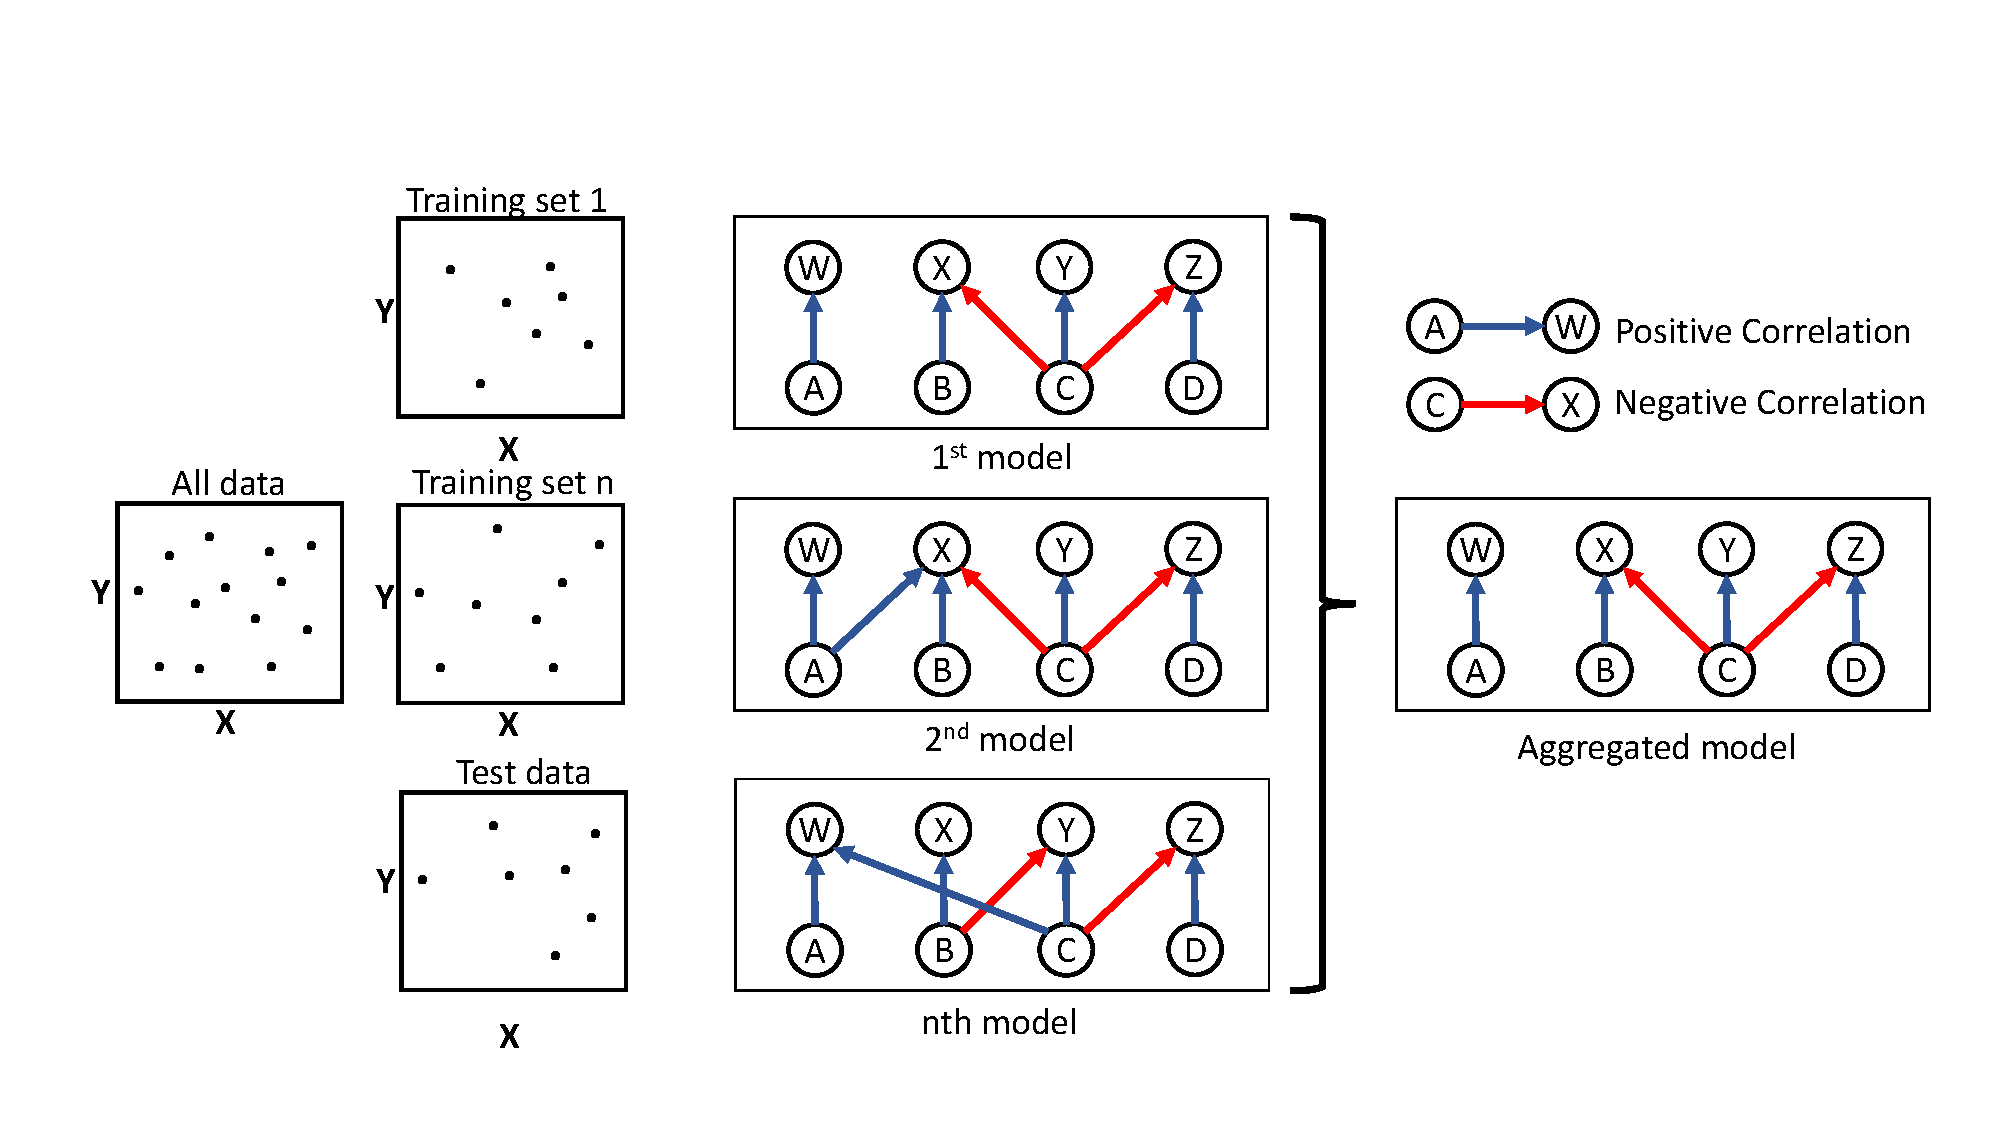
\includegraphics[width=14.0cm]{figs/bagging.pdf}
        \caption{Bagging or bootstrap aggregation}
        \label{fig:bg:bagging}
    \end{center}
\end{figure}

For online bagging approach $n \rightarrow \infty$, and the binomial distribution of $P(K=k)$ tends to a Poisson distribution with $P(K=k) = \exp(-1)/k!$. Using this justification, online bagging chooses a $k $ from $Poisson(1)$ for each incoming training examples $(x_i, y_i)$, and updates the base learning algorithms $k$ times. The classification is done as the same way of batched approach, by unweighted voting of $m$ base classifiers. For similar distribution of training examples, online bagging produces similar approximated base models. If (i) used base learner converges to the same classifier with increasing training examples, and (ii) base learner produces same classifier given a fixed training set for both batched and online bagging methods; then online bagging will converge to the classifier obtained though batched learning methods.


\subsection{Boosting}
Boosting is another supervised learning algorithm to iteratively improve learning hypothesis. The motivation behind the boosting approach is that a set of weak classifiers could create a single strong learner. It forces a weak classifier to update or generate new rules that make less mistakes on previously misclassified records. Initially all records are assigned same weights. At the end of a boosting round, weights might change due to the errors in classification. Weights of the instances are increased or decreased if they are classified wrongly or correctly, respectively. Thus successive classifiers depend upon their predecessors. 
\begin{figure}[htbp]
    \begin{center}
        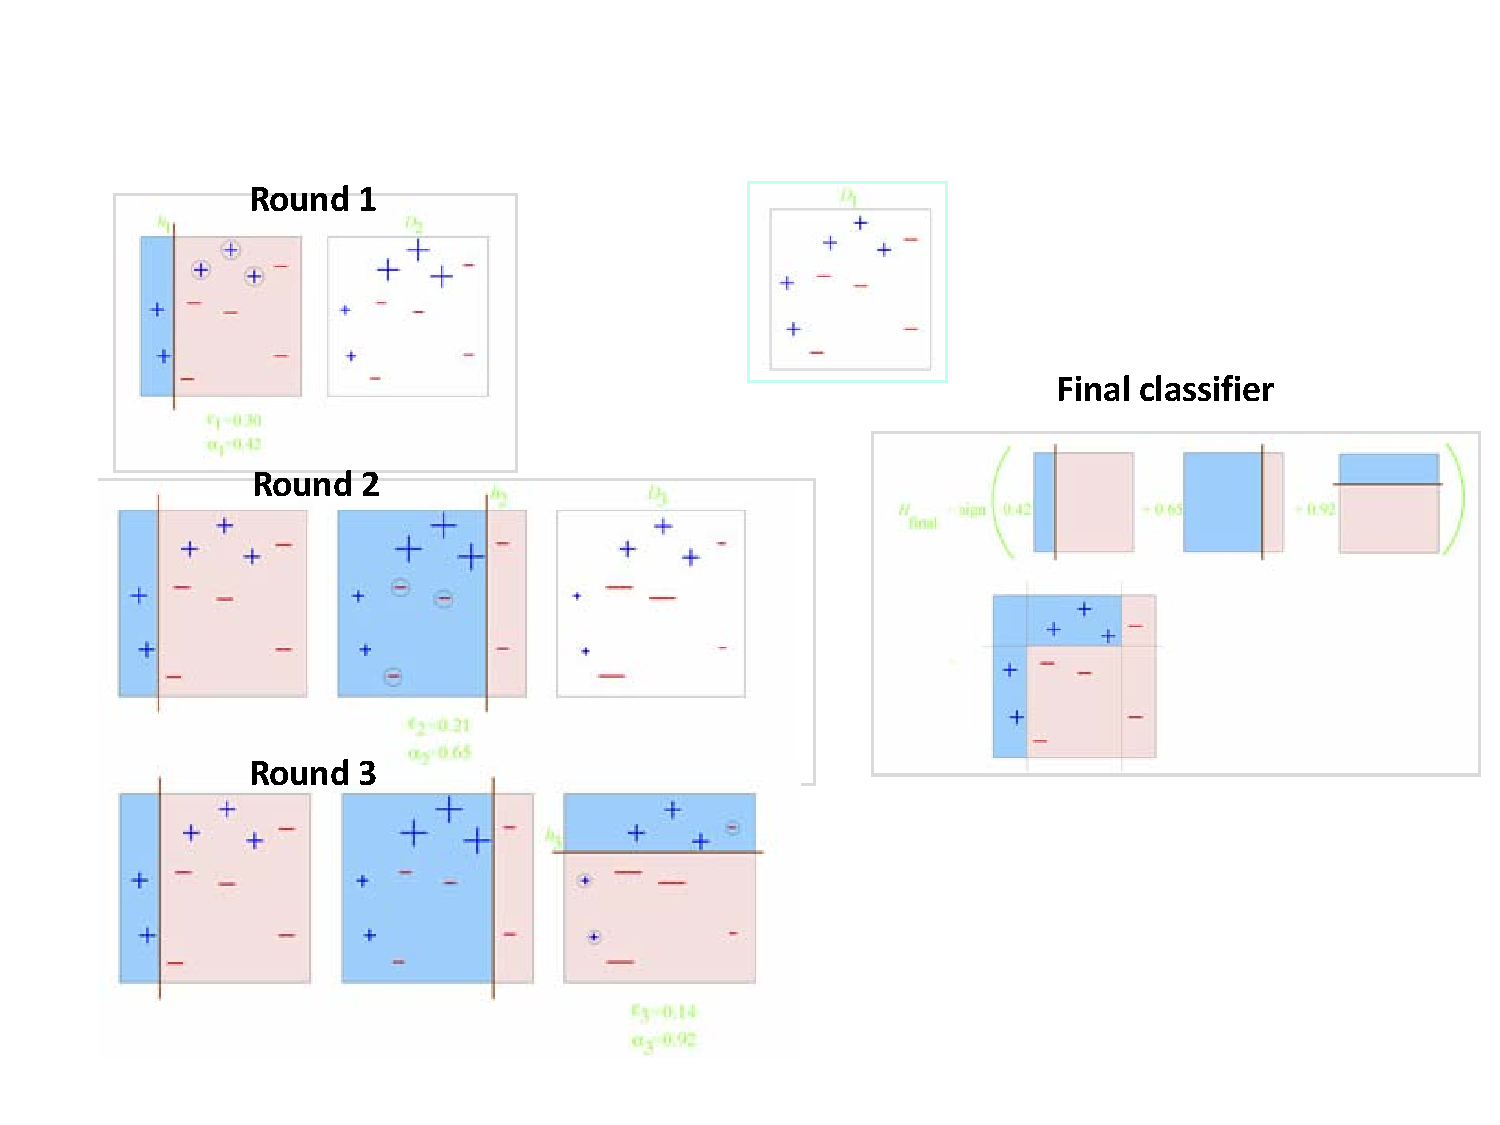
\includegraphics[width=12.0cm]{figs/boosting.pdf}
        \caption{Boosting method example}
        \label{fig:bg:bosting}
    \end{center}
\end{figure}

Mathematically, let $H= \{h_1, h_2, \dots, h_n\}$ be $n$ weak hypotheses. The combined hypothesis $H(.)$ is a weighted majority vote of the $n$ weak hypotheses where each hypothesis $h_i$ has a weight of $\alpha_i$ for $i = \{1, 2, \dots, n\}$:
\begin{equation}
\label{eqn:adaboostHypo}
    H(.) = sign \left(\sum_{i=1}^n \alpha_i h_i(x) \right).
\end{equation}

One of the earliest boosting approaches was proposed in~\cite{schapire90:whyens}. It calls weak learners three times on three modified distributions and achieves slight improvement in accuracy. Later,~\cite{freund97:boosting} proposed AdaBoost, an adaptive boosting method, that works with a principle of minimizing upper bound of empirical error. Let, $(x_1, y_1), (x_2, y_2), \dots, (x_n, y_n)$ are given examples where $x_i \in X, y_i \in Y = [-1, +1]$. Let, $D_t (i)$ be the weight of $i$-th example at $t$-th round. Then, AdaBoost initializes $D_1(i) =1/n$. Iterative steps are as follows:

For each iteration $t= 1, 2, \dots, T$:
\begin{itemize}
    \item Train weak learner using distribution $D_t$
    \item Get weak hypothesis $h_t : X \rightarrow \{-1, +1\}$ with error
    \[
        \epsilon_t = Pr_{i ~ D_t} [h_t(x_i) \ne y_i]
    \]
    \item Choose $\alpha_t = \frac{1}{2} \ln \left( \frac{1 - \epsilon_t}{\epsilon_t} \right)$
    \item Update $D_{t+1} (i) = \frac{D_t(i) \exp(-\alpha y_i h_t(x_i))}{Z_t}$ where $Z_t$ is a normalization factor
\end{itemize}
Finally, the output is calculated with the Equation~\ref{eqn:adaboostHypo} given above.

An online variant of AdaBoost uses a similar approach as online bagging method, simulating sampling with replacement using Poisson distribution. However, here the Poisson parameter $\lambda$ (Equation~\ref{eqn:poisson}) associated with an example is increased if that particular example is misclassified. In case of correct classification $\lambda$ is decreased. Similar to the AdaBoost, online boosting approach assigns total weights equally to the correctly and misclassified instances, i.e. half of the total weights each. Unlike AdaBoost, in online boosting weights are updated based on only the examples seen thus far rather than the complete training set. This is intuitively problematic as initial hypotheses are built on too few examples. Even with this limitation, online boosting shows good performance. Online boosting with na\"ive Bayes base learner converges to the model achieved with AdaBoost as the number of training instances tends to infinity.

\subsection{Adaptive-Size Hoeffding Tree (ASHT) Bagging}
\label{sec:bg:asht}
In previous section (Section~\ref{sec:bg:vfdt}), we have introduced Very Fast Decision Tree (VFDT) or Hoeffding Tree (HT). Hoeffding Tree is inspired by the fact that a small sample size could be sufficient to effectively choose an optimal splitting attribute. An upper bound of the error introduced because of such generalization is given using Hoeffding bound.

The Adaptive-Size Hoeffding Tree (ASHT) is, as the name suggests, extended from Hoeffding tree with deletion of nodes or resetting of the tree capabilities. Following are two significant differences of adaptive-size Hoeffding tree with Hoeffding tree: 
\begin{itemize}
    \item Maximum number of split nodes or the size of the tree is bounded in ASHT. There is no such limit on HT. HT grows indefinitely as the data and new concepts are introduced.
    \item When number of split nodes exceeds the maximum value (essentially after a new split), some nodes (or entire tree) are deleted to retain the tree property (max size).
\end{itemize}
There are two different choices for the deletion of nodes for the second point. First option is to delete the oldest node. In Hoeffding tree, root is always the oldest node. All children of root except for the nodes that were further splitted are also deleted in this case. The new root would be the node from the children of root not being deleted. Another and cruder approach would be to delete the complete tree altogether i.e. resetting the tree. 

\begin{figure}[htbp]
    \begin{center}
        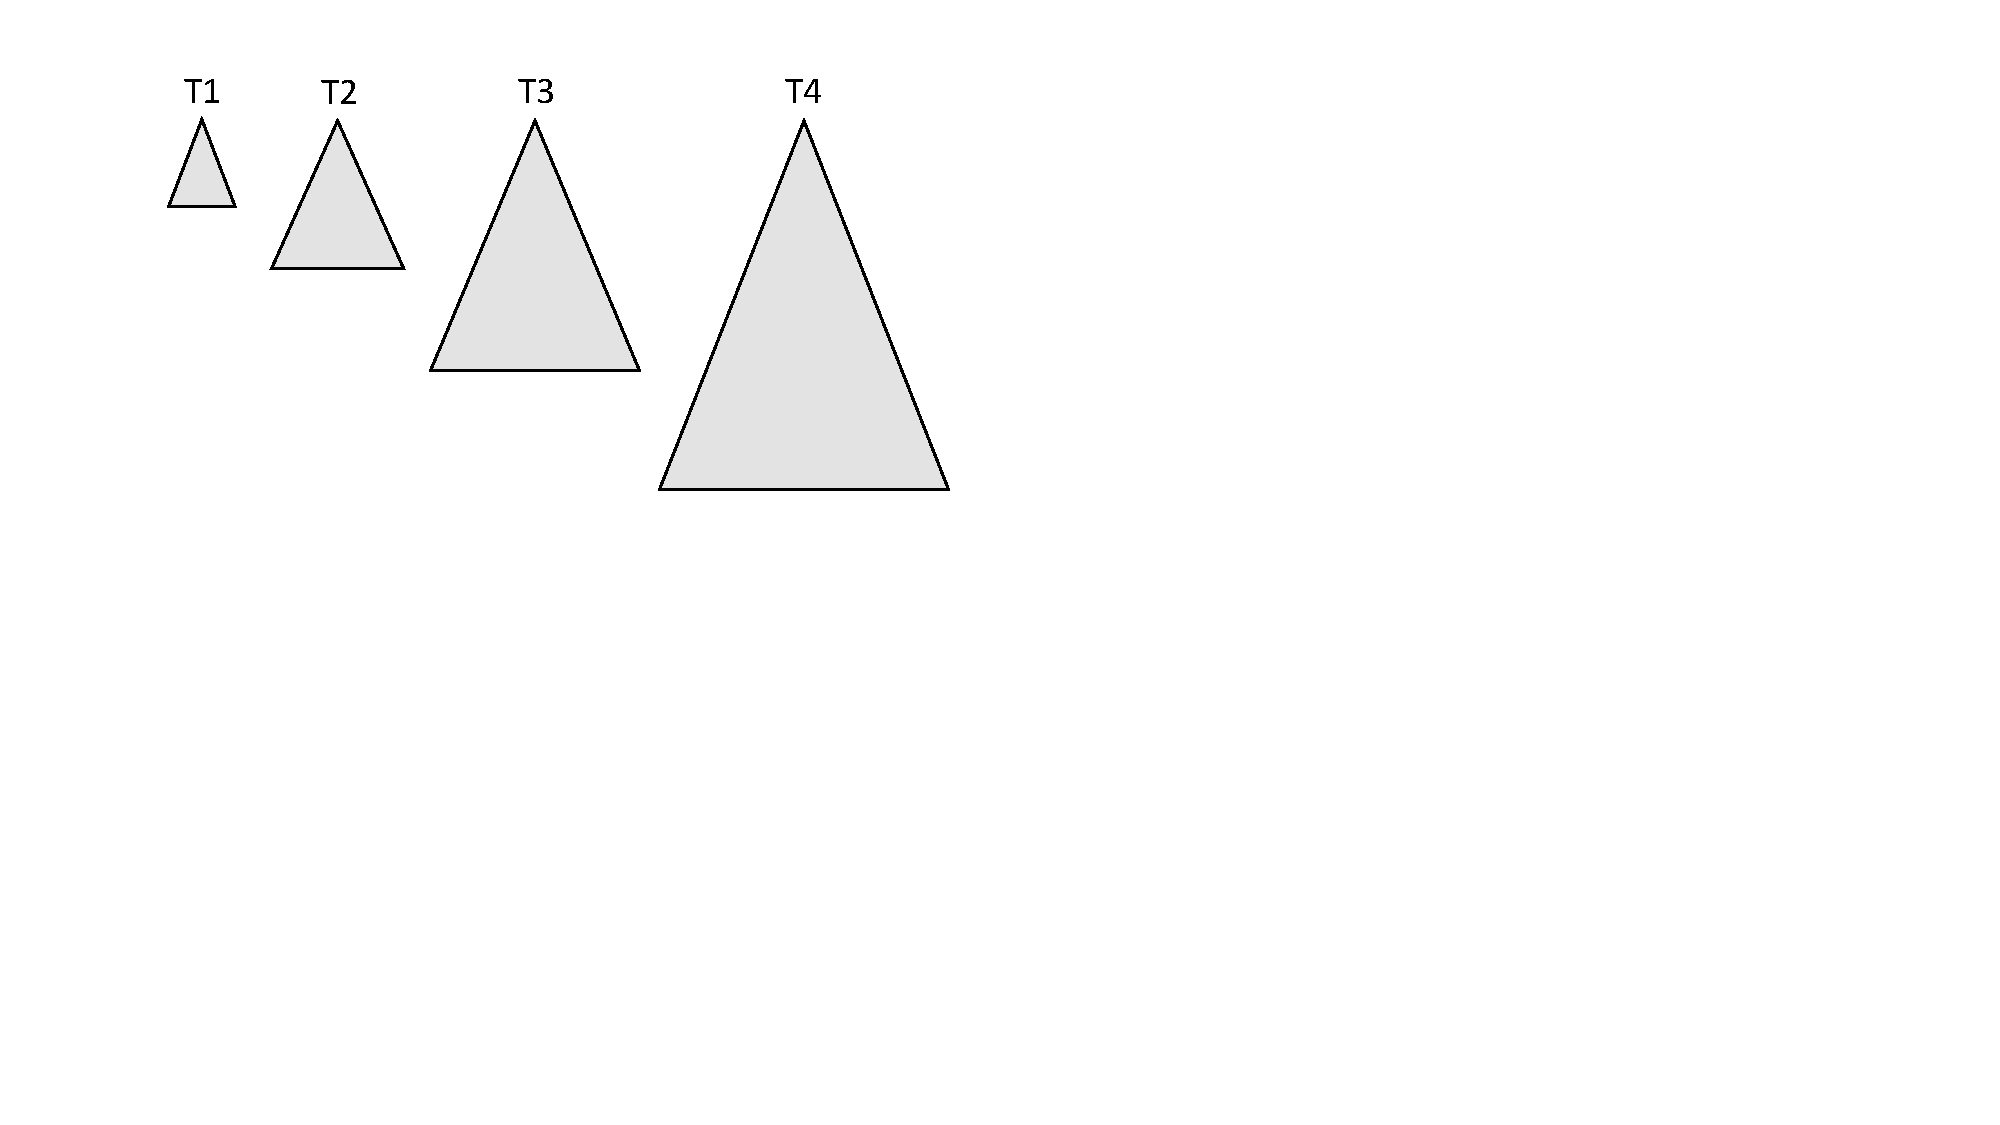
\includegraphics[width=10.0cm]{figs/ashtbagging.pdf}
        \caption{Adaptive Size Hoeffding Tree bagging concept}
        \label{fig:bg:asht}
    \end{center}
\end{figure}

Based on this modified Hoeffding tree, a bagging method is developed in~\cite{bifet09:asht}. The intuition of the method is as follows: smaller trees adapts to changes faster than the larger trees. However, larger trees perform better where data have only small changes or drifts because  they are built with more data. A tree of size $s$ would expect to be reset twice as often as a tree with size $2s$. Using an ensemble of different sizes would thus give a set of trees with different reset speeds. Smaller trees would be updated for small changes in the streams, while larger ones will maintain a history for longer period. Polling over this set of classifiers would thus expected to result in a classifier with finer granularity. It is to be noted that reset will occur even for stationary data, however, this should not have any negative influence on the ensemble's predictive performance for stationary cases.

The proposed bagging method in~\cite{bifet09:asht} uses $n$ adaptive-size Hoeffding trees. The $n$-th ASHT has twice the maximum size of $(n-1)$-th tree. Size of the smallest tree is 2. For the polling, each tree is associate with a weight, which is selected to be the inverse of squared error.

\subsection{ADWIN Bagging}
ADWIN Bagging combines three different powerful concepts together: (i) bagging (Section~\ref{sec:bg:bagging}), (ii) adaptive window change detection (Section~\ref{sec:bg:changedetection}), and (iii) Hoeffding tree (Section~\ref{sec:bg:vfdt}).

Bagging using ADWIN is implemented as ADWIN bagging where the bagging method is the online bagging method of Oza and Russell~\cite{oza01:obagboost} with the addition of the ADWIN algorithm as a change detector. Hoeffding Trees are used as base classifier. When a change is detected, the worst classifier of the ensemble  is removed and a new classifier is added to the ensemble. 
